The third prototype built as a proposal of the final TRITIUM detector module was TRITIUM-Aveiro, shown in Figure \ref{fig:TritiumAveiro0},designed and built in the workshop of the University of Aveiro. 

\begin{figure}[h]
\centering
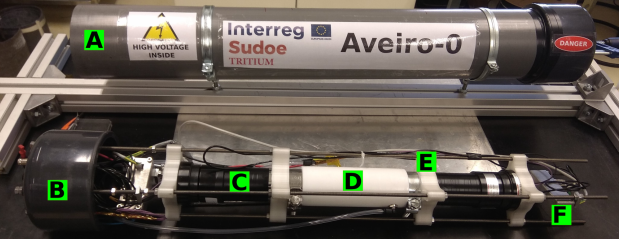
\includegraphics[scale=0.4]{5Prototypes/53FinalPrototypes/531TritiumAveiro/GeneralViewOfAveiroPrototype.png}
\caption{TRITIUM-Aveiro prototype.\label{fig:TritiumAveiro0}}
\end{figure}
This prototype consists of a Teflon vessel (marked as D in Figure \ref{fig:TritiumAveiro0}), shown in Figure \ref{fig:TeflonStructureFibersTritiumAveiro0}, with an internal cylindrical hole of $43~\mm$ diameter and $18~\cm$ length. 

\begin{figure}[h]
\centering
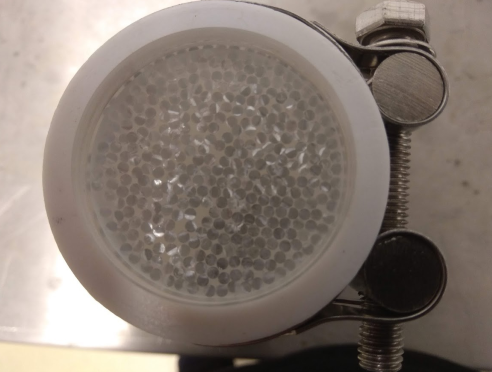
\includegraphics[scale=0.4]{5Prototypes/53FinalPrototypes/531TritiumAveiro/TeflonVessel_Fibers.png}
\caption{Teflon structure and fiber bundle used in TRITIUM-Aveiro prototype.\label{fig:TeflonStructureFibersTritiumAveiro0}}
\end{figure}
This vessel contains $360$ uncladded scintillating fibers of $180~\mm$ length. The fibers are BCF-10 from Saint-Gobain company \cite{DataSheetBCF10Fiber}, which have similar characteristics than the BCF-12 fibers, except the diameter, which is the double, $2~\mm$. A larger diameter is convenient because it facilitates the flow of water around the fibers, reducing problems related to surface tension and ensuring that the entire active volume of the fibers is used for tritium detection. In addition, a large radious increases the rigidity of the fiber. However, this large radious worsens the signal-to-background ratio. The detector active volume for $2~\mm$ fibers is smaller for the same volume, producing a smaller tritium signal and internal volume of the fibers unreachable by tritium decay electrons is larger, producing a larger background. As a result, a lower signal-to-background ratio is obtained. In order to quantify the importance of the fiber diameter, the measurements were compared with similar measurements performed with TRITIUM-IFIC 2 prototype, based on a similar configuration but with $1~\mm$ fibers.

The amount of fibers used in TRITIUM-Aveiro prototype is the maximum which allows the water to flow around the fibers, which are free inside the Teflon vessel. 

These fibers were cleaved with the device developed by TRITIUM but they were neither polished nor cleaned because the automatic polishing machine was not yet developed and it was not feasible to polish 360 fibers by hand. 

The Teflon vessel is totally closed and  a water inlet/outlet were installed in it to allow a constant water flux through it. Two PMMA $10~\mm$ thick windows, located at both ends of the fiber bundle, was used to read the fibers. Two clamps were used to make a tight junction of the Teflon walls and the PMMA. PMMA was chosen for its optical properties, especially its transmission coefficient, which is larger than $95\%$ at the working wavelength. Two PMTs (marked as C in Figure \ref{fig:TritiumAveiro0}) were used to read this prototype in time coincidence. HV was $-1500~\volt$, at which the quantum efficiency is $26\%$. PMTs were attached to both fiber bundle ends by two pieces (marked as E in Figure \ref{fig:TritiumAveiro0}) built with a 3D printer and they were optically coupled to the PMMA windows through optical grease \cite{OpticalGrease}. The PMTs used were R2154-02 2" from Hamamatsu \cite{DataSheetPMTsAveiro}, that have gain and efficiency quite similar to the PMTs used in the other prototypes.

This prototype and its electronics (marked as F in Figure \ref{fig:TritiumAveiro0}), were arranged in a structure, shown in Figure \ref{fig:TritiumAveiro0}, composed of several clamps and four long stainless-steel screws, locked to an external PVC structure, marked as A and B in Figure \ref{fig:TritiumAveiro0}, which protects the prototype from physical damage and provide a light-tight operation environment. This PVC structure is equiped with the necessary feed-through connectors.

Only one prototype was built, which was designed to be installed in the Arrocampo dam and its electronics, based on several PCBs, was specially designed, developed, built and tested to process and analyze the signals of this system, detailed in appendix \ref{App:ElectronicSystemAveiro}. Two interfaces were developed, one to control the PMT power supply, shown in Figure \ref{subfig:GUIHV}, and the other to control the different options of the electronics, such as thresholds and number of counts, shown in Figure \ref{subfig:GUIcounts}.

\begin{figure}
\centering
    \begin{subfigure}[b]{0.65\textwidth}
    \centering
    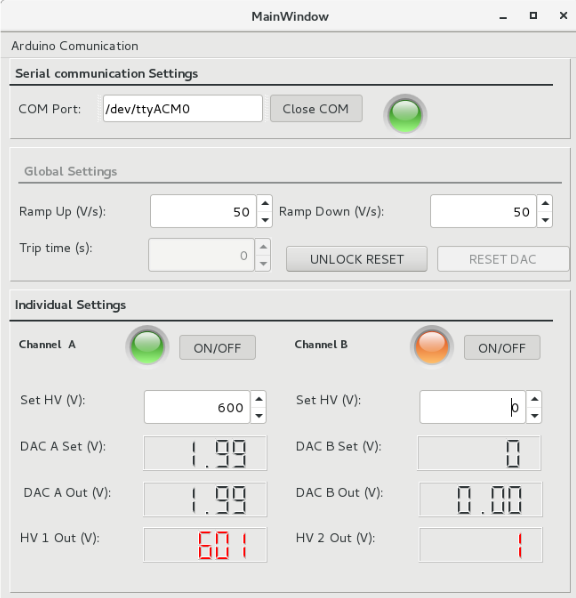
\includegraphics[width=\textwidth]{5Prototypes/53FinalPrototypes/531TritiumAveiro/GUIHVBoard.png}  
    \caption{\label{subfig:GUIHV}}
    \end{subfigure}
    \hfill
    \begin{subfigure}[b]{0.8\textwidth}
    \centering
    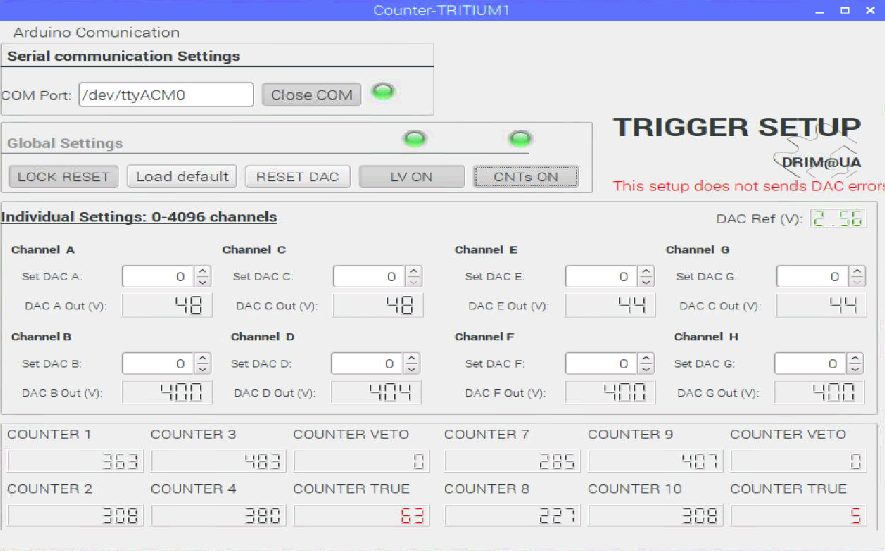
\includegraphics[width=\textwidth]{5Prototypes/53FinalPrototypes/531TritiumAveiro/CounterGUI.png}  
    \caption{\label{subfig:GUIcounts}}
    \end{subfigure}
 \caption{Graphical User Interface developed to control a) PMT HV employed. b) the counter system of the TRITIUM-Aveiro prototype}
 \label{fig:GUITRITIUMAveiro}
\end{figure}

Measurements taken in the laboratory were used to characterize the detector. For this task, the prototype was firstly filled with ultra-pure water, which was used to measure the background of the detector, and next, with a radioactive liquid tritium solution with an activity of $30~\kilo\becquerel/\liter$, which was used to mesure the efficiency and the low detection level of the prototype. The volume of ultrapure water and tritium solution used in TRITIUM-Aveiro prototype was $58~\milli\liter$. This prototype was installed in the Arrocampo dam to test its functionality and to begin with the tritium level monitoring. The laboratory and Arrocampo measurements are reported in chapter \ref{chap:ResultsPrototypes}.